O reino de ACM era comandado por um grande Rei que era obcecado por ordem. O
reino tinha forma retangular, e o rei dividiu o território em uma grade de
pequenos países retangulares. Antes de morrer, o Rei distribuiu os países entre
seus filhos.

No entanto, ele não sabe que seus filhos desenvolveram uma estranha rivalidade;
o primeiro herdeiro odiava o segundo herdeiro, mas não os demais; o segundo
herdeiro odiava o terceiro herdeiro, mas não os demais, e assim por diante.
Finalmente, o último herdeiro odiava o primeiro herdeiro, mas não os demais.

Logo que o Rei morreu, essa estranha rivalidade entre os filhos do Rei
desencadeou uma guerra generalizada no reino. Os ataques ocorriam apenas entre
pares de países adjacentes (que compartilham uma borda vertical ou horizontal).
Um país X atacava um país adjacente Y sempre que o proprietário de X odiava o
proprietário de Y. O país atacado era sempre conquistado pelo irmão atacante.
Por uma questão de honra, todos os ataques aconteciam simultaneamente, e um
conjunto de ataques simultâneos recebia o nome de batalha. Após um certo número
de batalhas, os filhos sobreviventes assinaram um tratado de trégua e nunca mais
batalharam.

Por exemplo, se o Rei tinha três filhos (0, 1 e 2) a figura abaixo mostra o que
acontece na primeira batalha dada uma distribuição inicial das terras:

\begin{center}
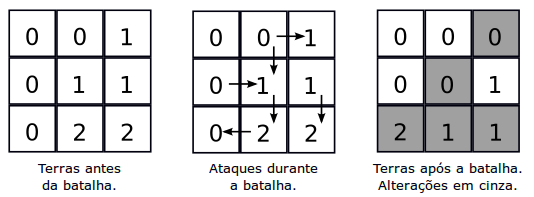
\includegraphics[scale=0.6]{problems/irmaos/imagens/irmaos.png}
\end{center}

Você foi contratado para ajudar um historiador da ACM a determinar, dados o
número de herdeiros, a distribuição inicial de territórios e o número de
batalhas, qual a distribuição final de territórios após as batalhas.

\subsection*{Entrada}

A entrada contém vários casos de teste. A primeira linha de um caso de teste
contém quatro inteiros N, R, C e K separados por um espaço em branco. N é o
número de herdeiros $(2 \leq N \leq 100)$, R e C são as dimensões do reino $(2
\leq R,C \leq 100)$ e K é o número de batalhas $(1 \leq K \leq 100)$. Herdeiros são
identificados por inteiros de 0 até N-1. Cada uma das seguintes R linhas contém
C inteiros $H_{r,c}$ separados por um espaço em branco, representando a distribuição
inicial de terras: $H_{r,c}$ é o proprietário inicial do país na linha $r$ e
coluna $c$ $(0 \leq H_{r,c} \leq N-1)$.

O último caso de teste é seguido de uma linha contendo quatro zeros separados
por um espaço em branco.

\subsection*{Saída}

Para cada caso de teste, seu programa deve imprimir R linhas com C inteiros
cada, separados por um espaço em branco, no mesmo formato da entrada,
representando a distrubuição das terras após todas as batalhas.

\begin{table}[!h]
\centering
\begin{tabular}{|l|l|}
\hline
\begin{minipage}[t]{3in}
\textbf{Exemplo de entrada}
\begin{verbatim}
3 4 4 3
0 1 2 0
1 0 2 0
0 1 2 0
0 1 2 2
4 2 3 4
1 0 3
2 1 2
8 4 2 1
0 7
1 6
2 5
3 4
0 0 0 0
\end{verbatim}
\vspace{1mm}
\end{minipage}
&

\begin{minipage}[t]{3in}
\textbf{Exemplo de saída}
\begin{verbatim}
2 2 2 0
2 1 0 1
2 2 2 0
0 2 0 0
1 0 3
2 1 2
7 6
0 5
1 4
2 3
\end{verbatim}
\vspace{1mm}
\end{minipage} \\
\hline
\end{tabular}
\end{table}

\newpage
